\section{氫原子(波耳氫原子模型)}

\begin{concept}
重點觀念:\\
氫原子是最簡單的電子－質子系統，因此能清楚呈現原子結構的基本原理。由於原子的能量是量子化的，電子只能存在於特定的能階上。當電子吸收或放出固定的能量時(在此為光子)，便會在不同能階之間轉換，此過程稱為躍遷，而記錄氫原子躍遷釋放出的光子，即可組成\underline{發射光譜}。
\end{concept}
\subsection{氫原子模型的出現}
拉塞福原子模型假設電子以圓周運動繞行原子核，然而電子會因加速度運動釋放電磁波，損失能量，最終掉入原子核。所以為了解決此困境，波耳提出了能階的概念，既電子繞行原子核的能量是不連續的(量子化)，從而解決了氫原子光譜困境。

\subsection{氫原子模型}
\subsubsection{基本假設}
\begin{itemize}
    \item 電子僅能在特定軌道上保持穩定狀態。
    \item 電子由高能階躍遷至低能階時，兩能階能量差以光子的形式放出。
    \item 電子角動量量子化：$mvr=n\hbar$。
\end{itemize}

\subsubsection{必背公式}

\begin{trick}
\textbf{1.氫原子能階公式}

\[
E_n=-\frac{13.6}{n^2} \text{ eV}
\]

電子由高能階 $n_i$ 躍遷至低能階 $n_f$ 時，放出的光子能量為
\[
\Delta E = E_i - E_f
\]

\vspace{0.3cm}

\textbf{2.芮得柏公式}

\[
\frac{1}{\lambda}=R_H
\left(
\frac{1}{n_f^2}-\frac{1}{n_i^2}
\right)
\]

其中
\[
R_H = 1.097\times10^{-2}\,nm^{-1}
\]

\textbf{記憶重點：}
能階差 $\rightarrow$ 決定光子的頻率與波長。
\end{trick}

\subsection{氫原子光譜系列}

\begin{enumerate}
    \item \textbf{萊曼系列}\quad <紫外線>：由 $n_i>1$ 的能階降至 $n_f=1$。
    
    \item \textbf{巴耳末系列} <可見光>：由 $n_i>2$ 的能階降至 $n_f=2$。
    
    \item \textbf{帕申系列}\quad<紅外線>：由 $n_i>3$ 的能階降至 $n_f=3$。
    
    \item \textbf{布拉克系列} <紅外線>：由 $n_i>4$ 的能階降至 $n_f=4$。
\end{enumerate}

\begin{figure}[H]
    \centering
    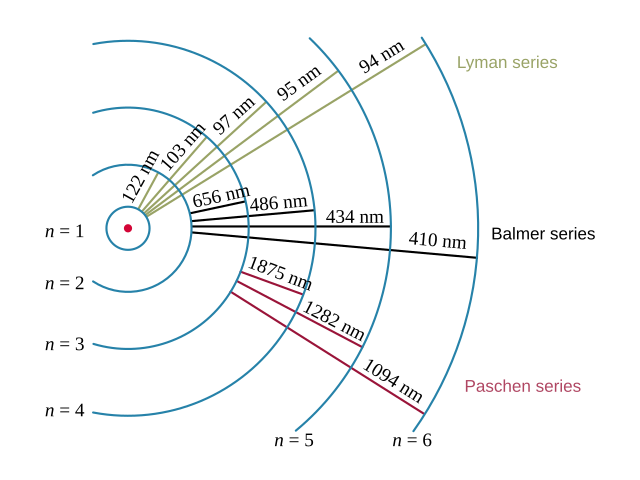
\includegraphics[width=0.6\linewidth]{graph/Hydrogen_transitions.svg.png}
    \caption{氫原子電子躍遷}
    \label{fig:氫原子圖}
\end{figure}

\subsection{波耳理論適用範圍}

\begin{trick}
波耳理論僅適用於\textbf{氫原子與單電子離子}  
（如 $He^+$、$Li^{2+}$、$Be^{3+}$ 等）。

對於原子序為 $Z$ 的單電子離子，其能階公式變為：

\[
E_n=-\frac{13.62}{n^2}\times Z^2\text{ eV}
\]

其中  \\
$Z$：原子序(原子核有幾顆質子) \\
$n$：主量子數

\textbf{記憶重點：}

能量與 $Z^2$ 成正比，核電荷越大，電子束縛越強。
\end{trick}